\documentclass[border=6pt]{standalone}
\usepackage[T1]{fontenc}
\usepackage[utf8]{inputenc}
\usepackage[scaled=0.98]{helvet}
\renewcommand{\familydefault}{\sfdefault}
\usepackage{amsmath}
\usepackage{graphicx}
\graphicspath{{../../../../../../exercises_lecturenotes/lecture_notes/kurs100_lektionsnoter/}}
\usepackage{tikz}
\usepackage{pgfplots}
\pgfplotsset{compat=1.18}
\usetikzlibrary{arrows.meta, decorations.pathreplacing, calc, positioning, fit, backgrounds, shapes.geometric}
\usepgfplotslibrary{groupplots,fillbetween}
\definecolor{scanpink}{HTML}{E5006D}
\definecolor{scanteal}{HTML}{00A6A6}
\definecolor{scannavy}{HTML}{243746}
\definecolor{scanlightgray}{HTML}{F1F2F3}
\begin{document}
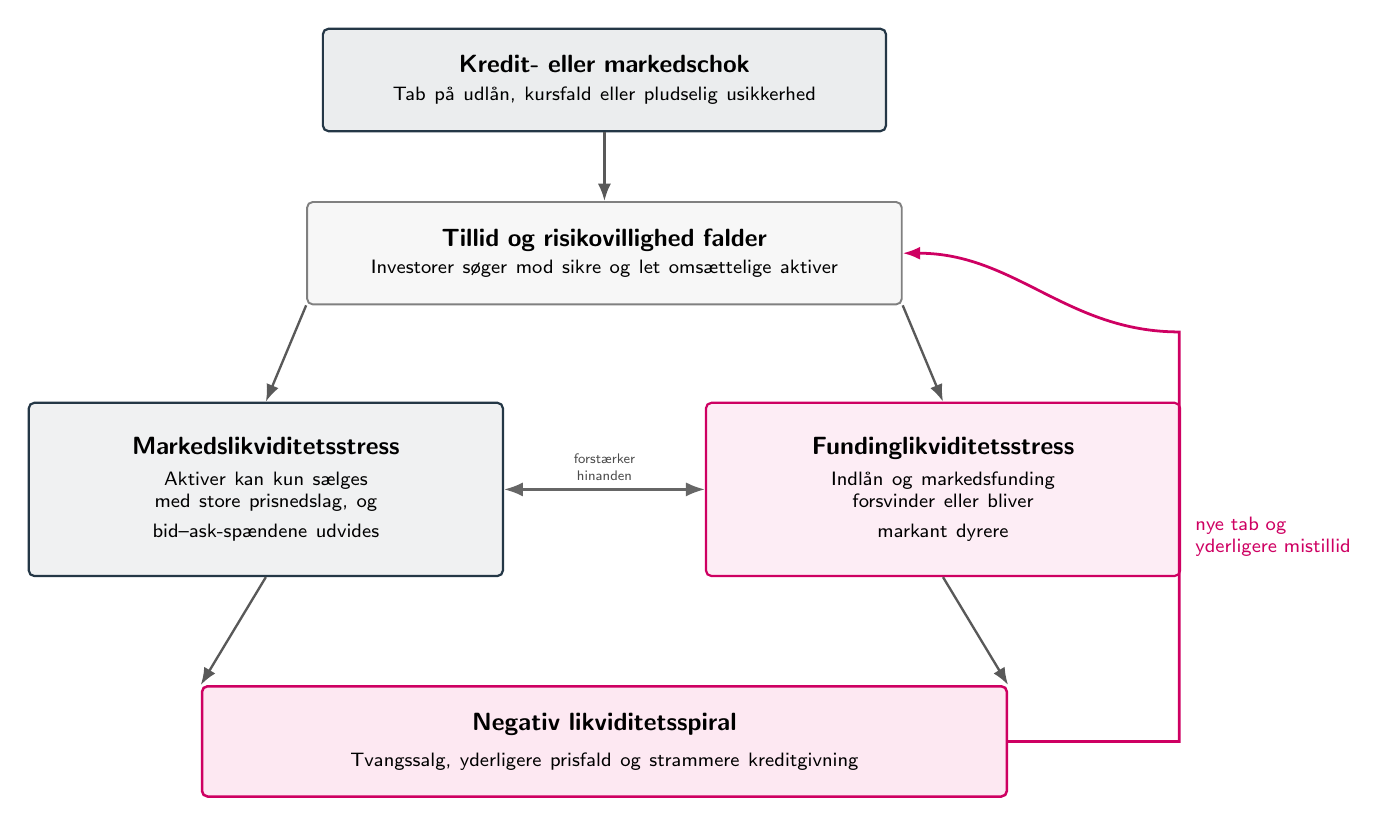
\begin{tikzpicture}[
    x=1cm,
    y=1cm,
    font=\small,
    shockbox/.style={
        draw=scannavy,
        fill=scannavy!9,
        rounded corners=2pt,
        line width=0.8pt,
        minimum height=13mm,
        text width=68mm,
        align=center,
        inner sep=5pt
    },
    confidencebox/.style={
        draw=black!50,
        fill=black!3,
        rounded corners=2pt,
        line width=0.7pt,
        minimum height=13mm,
        text width=72mm,
        align=center,
        inner sep=5pt
    },
    marketbox/.style={
        draw=scannavy,
        fill=scannavy!7,
        rounded corners=2pt,
        line width=0.8pt,
        minimum height=22mm,
        text width=56mm,
        align=center,
        inner sep=6pt
    },
    fundingbox/.style={
        draw=scanpink!90!black,
        fill=scanpink!7,
        rounded corners=2pt,
        line width=0.8pt,
        minimum height=22mm,
        text width=56mm,
        align=center,
        inner sep=6pt
    },
    spiralbox/.style={
        draw=scanpink!90!black,
        fill=scanpink!9,
        rounded corners=2pt,
        line width=0.9pt,
        minimum height=14mm,
        text width=98mm,
        align=center,
        inner sep=6pt
    },
    arr/.style={
        -{Latex[length=2.2mm]},
        draw=black!65,
        line width=0.85pt
    },
    interaction/.style={
        <->,
        >=Latex,
        draw=black!60,
        line width=0.85pt
    },
    feedback/.style={
        -{Latex[length=2.2mm]},
        draw=scanpink!90!black,
        line width=1pt
    }
]

% -----------------------------------------------------
% Noder
% -----------------------------------------------------

\node[shockbox] (shock) at (0,0)
{
    \textbf{Kredit- eller markedschok}\\[-1pt]
    \scriptsize
    Tab på udlån, kursfald eller pludselig usikkerhed
};

\node[confidencebox] (confidence) at (0,-2.2)
{
    \textbf{Tillid og risikovillighed falder}\\[-1pt]
    \scriptsize
    Investorer søger mod sikre og let omsættelige aktiver
};

\node[marketbox] (market) at (-4.3,-5.2)
{
    \textbf{Markedslikviditetsstress}\\[3pt]
    \scriptsize
    Aktiver kan kun sælges\\
    med store prisnedslag, og\\
    bid--ask-spændene udvides
};

\node[fundingbox] (funding) at (4.3,-5.2)
{
    \textbf{Fundinglikviditetsstress}\\[3pt]
    \scriptsize
    Indlån og markedsfunding\\
    forsvinder eller bliver\\
    markant dyrere
};

\node[spiralbox] (spiral) at (0,-8.4)
{
    \textbf{Negativ likviditetsspiral}\\[2pt]
    \scriptsize
    Tvangssalg, yderligere prisfald og strammere kreditgivning
};

% -----------------------------------------------------
% Hovedforløb
% -----------------------------------------------------

\draw[arr] (shock) -- (confidence);

\draw[arr] (confidence.south west) -- (market.north);
\draw[arr] (confidence.south east) -- (funding.north);

% Interaktion mellem de to bokse
\draw[interaction] (market.east) -- (funding.west)
    node[
        midway,
        yshift=8pt,
        fill=white,
        inner sep=1.5pt,
        font=\tiny,
        align=center,
        text=black!70
    ]
    {forstærker\\hinanden};

\draw[arr] (market.south) -- (spiral.north west);
\draw[arr] (funding.south) -- (spiral.north east);

% -----------------------------------------------------
% Feedback-loop uden at ramme boksene
% -----------------------------------------------------

\coordinate (fb1) at (7.3,-8.4);
\coordinate (fb2) at (7.3,-3.2);

\draw[feedback]
    (spiral.east) -- (fb1)
    -- node[
        right,
        font=\scriptsize,
        align=left,
        text=scanpink!90!black,
        xshift=2pt
    ]
    {nye tab og\\yderligere mistillid}
    (fb2)
    to[out=180,in=0] (confidence.east);

\end{tikzpicture}
\end{document}
